\documentclass[11pt,a4paper]{article}
\usepackage[utf8]{inputenc}
\usepackage[T1]{fontenc}
\usepackage[spanish,es-nodecimaldot,es-tabla]{babel}
\usepackage{lmodern}
\usepackage[margin=2.3cm]{geometry}
\usepackage{amsmath,amssymb}
\usepackage{graphicx}
\usepackage{booktabs}
\usepackage{longtable}
\usepackage{float}
\usepackage{array}
\usepackage{caption}
\usepackage{enumitem}
\usepackage{xcolor}
\usepackage{multirow}
\usepackage[most]{tcolorbox}
\usepackage[hidelinks]{hyperref}
\usepackage{url}
\urlstyle{same}
\captionsetup{font=small,labelfont=bf}
\setlist{itemsep=1pt,topsep=3pt}
\sloppy
\newcommand{\Erms}{E_{\mathrm{rms}}}
\newcommand{\emx}{e_{\max}}
\newtcolorbox{caja}[1]{colback=gray!8,colframe=gray!60,title={#1},fonttitle=\bfseries,coltitle=black,colbacktitle=gray!20}

\title{\textbf{Ajuste de curvas tipo J}}
\author{Santiago y Pablo}
\date{27 de noviembre de 2026}
\begin{document}
\maketitle

\begin{abstract}
\noindent Se presenta un método para ajustar una curva creciente y convexa ---una curva en J--- dada en un intervalo. La curva se aproxima como una suma de rectas truncadas $S_j\max(0,x-k_j)$, con nudos $k_j$ y pendientes $S_j$ fijos y coeficientes enteros no negativos, de 0 a 20. La base de rectas se elige una sola vez para toda una familia de curvas, con tres criterios: precisión en las peores curvas, buen condicionamiento numérico y coeficientes no negativos. Para cada curva, los coeficientes enteros que minimizan el peor error (diseño \emph{minimax}) se obtienen exactamente por programación lineal entera. Con esos ajustes se entrena una red neuronal que, una vez entrenada, da los coeficientes de una curva nueva en una sola evaluación, sin optimizar. Si a las variables se les da nombre físico ---estiramiento circunferencial en abscisas y tensión circunferencial en ordenadas---, la curva es la respuesta tensión--estiramiento de una pared arterial, cada recta es un material tipo fibra y cada coeficiente es un número de láminas. Con las curvas de 41 carótidas humanas (Masson et al.) y 6 rectas, la red, con una revisión de $\pm1$ en cada coeficiente, ajusta con un peor error de 3\,\% del rango o menos los 31 sujetos con que se entrenó, los 10 de prueba y 50 de 63 curvas de otros tres estudios; el ajuste minimax, que es el techo de lo alcanzable con coeficientes enteros, 57 de esas 63.
\end{abstract}

%=====================================================================
\section{El problema}
Sea $y(x)$ una curva dada en $n$ puntos $x_1<\dots<x_n$ de un intervalo $[a,b]$, creciente y convexa: una curva en J, plana al comienzo y empinada al final. Se busca representarla con pocos parámetros, de modo que
\begin{enumerate}[label=(\roman*)]
\item el ajuste conserve la forma: creciente y convexo, como la curva;
\item el error se controle en el peor punto, no solo en promedio;
\item los parámetros tomen valores en un conjunto finito y pequeño (enteros de 0 a 20), porque cada uno representa una cantidad que se fabrica en unidades;
\item la misma representación sirva para toda una familia de curvas, y el ajuste de una curva nueva sea inmediato.
\end{enumerate}
La herramienta resultante es una red neuronal entrenada dentro del rango de esa familia: recibe la curva y devuelve sus coeficientes en una evaluación.

%=====================================================================
\section{La representación: una base de rectas truncadas}
La función base $j$ es una recta truncada:
\begin{equation}\label{eq:base}
A_j(x)=S_j\,\max(0,\ x-k_j):
\end{equation}
vale cero hasta su \emph{nudo} $k_j$ y desde ahí crece con pendiente $S_j>0$. La curva se aproxima por
\begin{equation}\label{eq:ajuste}
\hat y(x)=\sum_{j=1}^{N}z_j\,A_j(x)=(Az)(x),\qquad z_j\in\{0,1,\ldots,20\},
\end{equation}
con $A\in\mathbb R^{n\times N}$ la matriz de la base (una fila por punto $x_i$, una columna por recta). Cada nudo produce un quiebre en el que la pendiente aumenta en $z_jS_j$; con pocos nudos bien ubicados, la suma arma la J (Fig.~\ref{fig:ejbase}).

\textbf{La forma se conserva por construcción.} Cada $A_j$ es no decreciente y convexa, y una combinación con coeficientes no negativos de funciones no decrecientes y convexas también lo es: todo ajuste~\eqref{eq:ajuste} es una curva en J, poligonal. Para nudos fijos, además, $\hat y$ es \textbf{lineal} en los coeficientes.

\begin{figure}[tb]\centering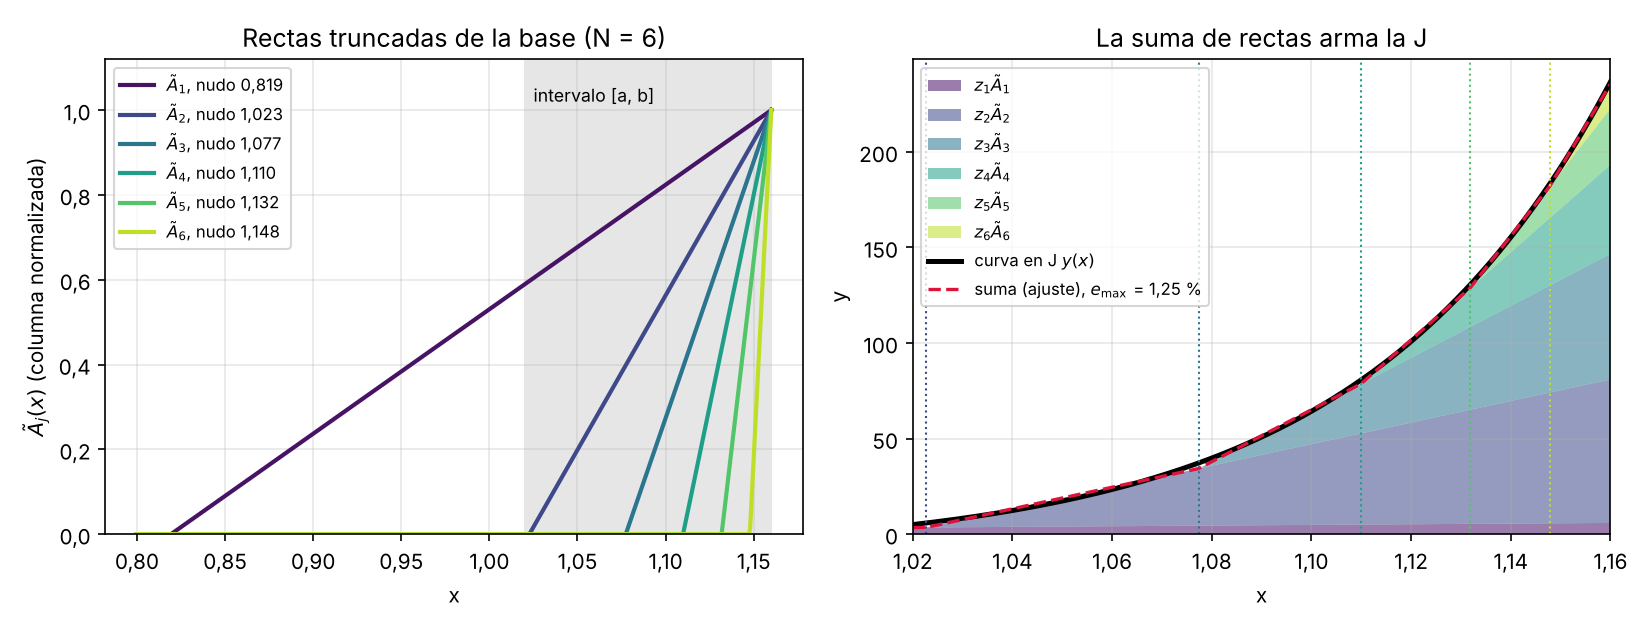
\includegraphics[width=\textwidth]{base_ejemplo.png}
\caption{Izquierda: las 6 rectas truncadas de la base usada en la Sección~\ref{sec:aplic}, con cada columna dividida por su máximo, de modo que todas valen 1 en $x=b$; la primera tiene su nudo antes del intervalo. Derecha: ajuste por mínimos cuadrados de una curva en J de prueba, $y=5+15\,(e^{20(x-1{,}02)}-1)$; cada franja de color es el aporte $z_j\tilde A_j$ de una recta, y su suma (rojo) sigue la curva (negro). Las líneas punteadas marcan los nudos.}\label{fig:ejbase}\end{figure}

\textbf{Error.} Para una curva con rango $\Delta=\max y-\min y$,
\begin{equation}\label{eq:emax}
e_{\max}=\frac{100}{\Delta}\max_i\,\lvert y_i-\hat y_i\rvert\quad[\%],\qquad E_{\mathrm{rms}}=\frac{100}{\Delta}\Bigl(\frac1n\sum_i(y_i-\hat y_i)^2\Bigr)^{1/2}.
\end{equation}
$e_{\max}$ es el peor punto, en porcentaje del rango, y es tan exigente con una curva de poco recorrido como con una de mucho. \textbf{Meta: $e_{\max}\le3$\,\%.}

%=====================================================================
\section{Elección de la base}
Los nudos $k=(k_1,\ldots,k_N)$ se eligen \textbf{una sola vez, para toda la familia de curvas}, minimizando una función de costo $\Phi(k)$ evaluada sobre un conjunto grande de curvas representativas de la familia (aquí, 22\,500 curvas y los 31 sujetos de entrenamiento). $\Phi$ reúne tres exigencias: precisión en las peores curvas, buen condicionamiento y coeficientes no negativos.

\subsection{Precisión en las peores curvas}
Para cada curva de la familia se calcula el $e_{\max}$ de su ajuste por mínimos cuadrados. Eso da una distribución de errores, una por curva, y hay que resumirla en un número.

\paragraph{Qué es el CVaR.} El CVaR (\emph{conditional value at risk}, valor en riesgo condicional) es una medida de la cola de una distribución, tomada de la gestión de riesgo financiero~\cite{rockafellar}. Para una variable aleatoria $X$ ---aquí, el $e_{\max}$ de una curva de la familia--- y un nivel $\alpha$, es el valor medio de $X$ en la fracción $1-\alpha$ de los casos peores:
\begin{equation}\label{eq:cvar}
\mathrm{CVaR}_\alpha(X)=\min_{t}\Bigl\{\,t+\frac{1}{1-\alpha}\,\mathbb E\bigl[\max(0,\,X-t)\bigr]\Bigr\},
\end{equation}
donde el $t$ que minimiza es el cuantil $\alpha$ de $X$. Con $M$ curvas se calcula sin optimizar: se ordenan los $e_{\max}$ de mayor a menor y se promedian los $\lceil(1-\alpha)M\rceil$ primeros. Aquí $\alpha=0{,}99$ y la muestra tiene 2532 curvas (2500 de la familia, los 31 sujetos de entrenamiento y la curva límite superior; paso~3 de la metodología, más abajo), de modo que $\mathrm{CVaR}_{99}$ es \textbf{el promedio de los $e_{\max}$ de las 26 peores curvas}.

\paragraph{Por qué el CVaR.} El CVaR está entre los dos resúmenes obvios. El promedio de todas las curvas ($\alpha=0$) dejaría sin control a las peores, que son las que deciden si se cumple la meta. El máximo ($\alpha\to1$) haría depender la elección de una única curva, y una sola curva rara cambiaría la base. El CVaR mira las peores sin depender de una sola. Se suma un término menor, 0,25 veces el $E_{\mathrm{rms}}$ medio, para que mejore también el ajuste típico.

\subsection{Condicionamiento: el criterio $\kappa(A)<30$}
\paragraph{Definición.} Sea $\tilde A$ la matriz de la base con cada columna dividida por su máximo:
\[
\tilde A_{ij}=\frac{\max(0,\,x_i-k_j)}{b-k_j}.
\]
Como cada recta es creciente, su máximo está en el extremo derecho $x=b$, y ahí todas las columnas valen 1 (Fig.~\ref{fig:ejbase}, izquierda). La descomposición en valores singulares~\cite{golub} escribe $\tilde A=U\Sigma V^{\top}$, con $U$ ($n\times N$) y $V$ ($N\times N$) de columnas ortonormales y $\Sigma$ diagonal con los valores singulares $s_1\ge\dots\ge s_N\ge0$, que son las raíces cuadradas de los autovalores de $\tilde A^{\top}\tilde A$. El mayor y el menor tienen un sentido directo:
\[
s_{\max}=\max_{\lVert v\rVert=1}\lVert\tilde Av\rVert,\qquad s_{\min}=\min_{\lVert v\rVert=1}\lVert\tilde Av\rVert:
\]
cuánto se estira y cuánto se encoge, como mucho, un vector de coeficientes al convertirse en curva. El número de condición es su cociente,
\begin{equation}\label{eq:kappa}
\kappa(A)=\frac{s_{\max}(\tilde A)}{s_{\min}(\tilde A)},
\end{equation}
y mide cuán distintas son esas dos situaciones extremas~\cite{trefethen}. Se normalizan las columnas porque las pendientes $S_j$ son una escala arbitraria (la unidad de cada recta): normalizadas, $\kappa$ depende solo de dónde están los nudos.

\paragraph{Qué mide.} Para mínimos cuadrados con residuo chico, como aquí (menos del 1,5\,\% del rango), una perturbación relativa de la curva se traslada a los coeficientes amplificada a lo sumo, a primer orden, por un factor del orden de $\kappa$~\cite{golub}:
\[
\frac{\lVert\delta z\rVert}{\lVert z\rVert}\lesssim\kappa(A)\,\frac{\lVert\delta y\rVert}{\lVert y\rVert}.
\]
Geométricamente, $s_{\min}$ chico significa que existe una combinación de columnas casi nula: dos o más rectas casi paralelas en el intervalo. Ocurre cuando dos nudos están muy cerca. Entonces el ajuste puede sumar mucho de una recta y restar casi lo mismo de la otra sin que la curva cambie: los coeficientes quedan mal determinados y aparecen valores grandes de signo opuesto que se compensan.

\paragraph{Un ejemplo.} Con una curva en J de prueba, $y=5+15\,(e^{20(x-1{,}02)}-1)$ en $[1{,}02;\,1{,}16]$, y la base de 6 rectas de la Tabla~\ref{tab:bases}, $\kappa=28$, los seis coeficientes del ajuste son positivos y un ruido de 1\,\% en la curva los mueve como mucho un 5\,\%. Si se acerca el nudo 5 a 0,003 del nudo 4, $\kappa$ sube a 143: el coeficiente 4 pasa a ser negativo ($-34$, en unidades de la columna normalizada) y el 5 se triplica (de 29 a 99), y el mismo ruido mueve el coeficiente 4 un 9\,\%. La curva ajustada casi no cambia, pero los coeficientes ya no tienen sentido.

\paragraph{Por qué importa aquí.} Un coeficiente mal determinado es un problema por tres razones: (1) puede salir negativo, y eso rompe la convexidad garantizada y no se fabrica; (2) al pasar a enteros, una unidad en una dirección mal condicionada mueve mucho la curva; y (3) la red debe aprender la relación curva $\to$ coeficientes, y una relación que amplifica mucho las diferencias entre curvas es más difícil de aprender.

\paragraph{Por qué 30 y qué limita.} El umbral es una elección de diseño, no sale de un teorema: con un error de 1\,\% en la curva, acota en el peor caso en 30\,\% el error relativo de los coeficientes, y en la práctica, como en el ejemplo, el error es mucho menor. $\kappa$ crece cuando los nudos se acercan y, por lo tanto, cuando se ponen más rectas en el mismo intervalo. La Fig.~\ref{fig:cond} lo muestra con dos cálculos hechos para este trabajo: correr un nudo hacia otro en la base de 6 rectas, y repartir $N$ nudos en partes iguales. Con nudos equiespaciados, 6 rectas ya superan el umbral ($\kappa=46$); la búsqueda ubica los nudos de modo que 6 rectas quedan en 28,0 y 5 en 19,0. Así, el umbral es, junto con la precisión, lo que limita cuántas rectas caben en el intervalo.

\paragraph{Cómo se impone.} De dos maneras: una separación mínima de 0,008 entre nudos, como restricción dura, y un término de penalización en $\Phi$, $50\,\max\bigl(0,\ \kappa-29\bigr)$, que empieza a actuar una unidad antes del umbral para dejar margen. La separación mínima sola no alcanza (en el ejemplo de la Fig.~\ref{fig:cond}, con 0,008 de separación $\kappa\approx57$); es la penalización la que lleva la base por debajo de 30.

\begin{figure}[tb]\centering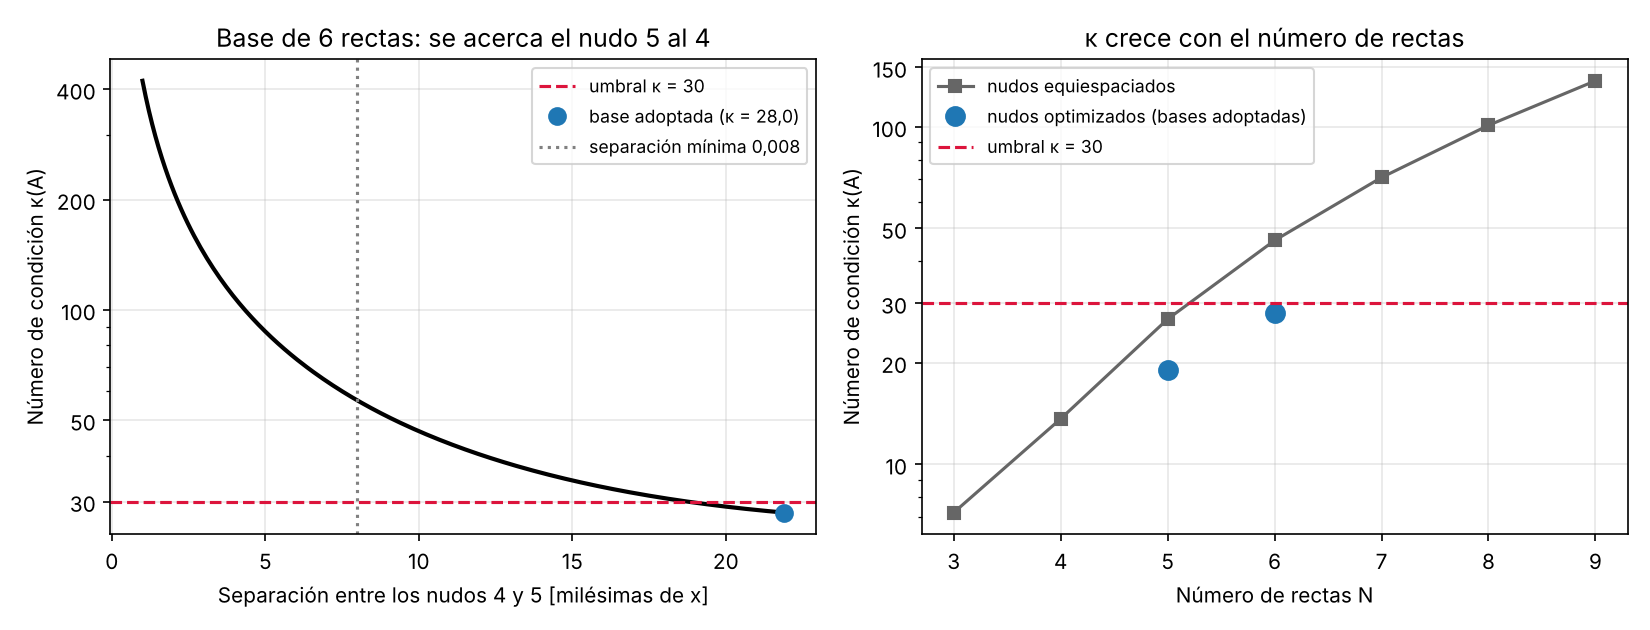
\includegraphics[width=\textwidth]{condicion_base.png}
\caption{Número de condición~\eqref{eq:kappa}, calculado para este trabajo con 999 puntos en $[1{,}02;\,1{,}16]$. Izquierda: en la base de 6 rectas de la Tabla~\ref{tab:bases} se dejan fijos todos los nudos salvo el 5, que se corre hacia el 4, $k_5=k_4+d$, con la separación $d$ de 0,001 a 0,0219 (la de la base adoptada); $\kappa$ crece rápidamente al juntarse los nudos. Derecha: bases sin optimizar, con $k_1=0{,}82$ y $k_2,\ldots,k_N$ equiespaciados entre 1,023 y 1,148 (cuadrados); puntos azules: las bases optimizadas de la Tabla~\ref{tab:bases}. Con nudos equiespaciados, $\kappa$ supera el umbral desde $N=6$; con los nudos optimizados, 6 rectas quedan debajo.}\label{fig:cond}\end{figure}

\subsection{Coeficientes no negativos}
El ajuste libre por mínimos cuadrados no debe necesitar coeficientes negativos en ninguna curva de la familia: un coeficiente negativo rompería la convexidad garantizada y no corresponde a ninguna cantidad fabricable. Se exige en las 22\,500 curvas, en los sujetos de entrenamiento y en las curvas límite, con una tolerancia de 0,01 unidad. Como el signo de un coeficiente no cambia al escalar su columna, esta condición queda fijada por los nudos.

\subsection{La función de costo y su minimización}
Con todo,
\begin{equation}\label{eq:costo}
\Phi(k)=\mathrm{CVaR}_{99}(e_{\max})+0{,}25\,\overline{E_{\mathrm{rms}}}+50\,\max\bigl(0,\ \kappa(A)-29\bigr)+1000\,\overline{n^{-}},
\end{equation}
con $\overline{n^{-}}$ el promedio, sobre las curvas, de $n^{-}=\sum_j\max\bigl(0,\,-10\,z_j/z_j^{\max}\bigr)$: la suma de los coeficientes negativos de una curva, medidos en décimas del mayor valor $z_j^{\max}$ que toma ese coeficiente en la familia.

\paragraph{De dónde sale y cómo se justifica.} $\Phi$ convierte las tres exigencias en un solo número a minimizar. El primer par de términos es el \emph{objetivo}: la precisión. Los otros dos son \emph{restricciones}, impuestas por penalización exterior~\cite{nocedal}: valen cero mientras se cumplen y crecen en cuanto se violan. Los pesos no se deducen de un principio: se eligen por escala, para que cada término cumpla su papel. El CVaR y el $E_{\mathrm{rms}}$ están en porcentaje del rango y valen unos pocos puntos (1 a 3), y en esa escala:
\begin{itemize}
\item \textbf{0,25} hace del $E_{\mathrm{rms}}$ un criterio secundario: desempata entre bases de CVaR parecido sin imponerse sobre él;
\item \textbf{50} por unidad de $\kappa$ por encima de 29: pasar de 29 a 30 ya cuesta 50 puntos, más que cualquier mejora de precisión posible, así que el mínimo de $\Phi$ nunca está en una base con $\kappa\ge30$;
\item \textbf{1000} por décima de coeficiente negativo: un coeficiente negativo de solo el 0,1\,\% de su máximo, si aparece en todas las curvas, ya cuesta 10 puntos.
\end{itemize}
Con estos pesos, el mínimo de $\Phi$ es la base más precisa entre las que cumplen $\kappa<30$ y no necesitan coeficientes negativos: las penalizaciones hacen de restricciones. Por eso el último paso de la metodología verifica que la base obtenida las cumpla de verdad. Las restricciones geométricas (separación y límites de los nudos) son, en cambio, duras: si un juego de nudos las viola, $\Phi=10^{9}$ y se descarta.

\begin{caja}{Metodología de elección de la base}
\begin{enumerate}[label=\arabic*.]
\item \textbf{Fijar $N$} y las restricciones: $k_1$ antes del intervalo (aquí entre 0,6 y 0,98); $k_2,\ldots,k_N$ entre 1,00 y $b-0{,}012$, separados al menos 0,008. El último queda así a más de 0,012 del extremo $b$, para que su recta actúe en suficientes puntos.
\item \textbf{Generar la familia}: curvas representativas dentro de la franja (aquí, 22\,500 de la ley de Masson con parámetros de los sujetos de entrenamiento mezclados, perturbados o sorteados) y los sujetos de entrenamiento. Los sujetos de prueba no intervienen.
\item \textbf{Para cada candidato $k$}: armar $\tilde A$ y calcular $\kappa$ por SVD; ajustar por mínimos cuadrados una muestra de la familia (2500 curvas, los sujetos y la curva límite superior, en uno de cada dos puntos, para abaratar) y calcular el CVaR 99\,\% de $e_{\max}$ y el $E_{\mathrm{rms}}$ medio; contar los coeficientes negativos en toda la familia; evaluar $\Phi$.
\item \textbf{Minimizar $\Phi$}: evolución diferencial~\cite{storn} (hasta 300 generaciones, tolerancia $10^{-6}$), que no usa derivadas y explora todo el dominio sin quedarse en el primer mínimo local, y refinamiento con el simplex de Nelder--Mead~\cite{nelder} (hasta 6000 iteraciones).
\item \textbf{Fijar las pendientes}: $S_j=\mathrm{PEND}_{\max,j}/20$, con $\mathrm{PEND}_{\max,j}$ la mayor pendiente que la recta $j$ debe aportar en la familia (calculada con la seudoinversa), para que ninguna curva necesite más de 20 unidades.
\item \textbf{Verificar}: $\kappa<30$ y ningún coeficiente negativo en la familia.
\end{enumerate}
\end{caja}

Las bases que resultan para la aplicación están en la Tabla~\ref{tab:bases} y en las Figs.~\ref{fig:ejbase} y~\ref{fig:bases}.

\paragraph{El primer nudo antes del intervalo.} $[a,b]$ es el intervalo en que están dadas las curvas; en la aplicación, $a=1{,}02$ y $b=1{,}16$. En $x=a$ las curvas de la familia ya valen más que cero (de 4,7 a 49\,kPa en la aplicación). Una recta con nudo $k_j\ge a$ vale cero en $x=a$, así que ese valor solo puede darlo una recta con el nudo antes de $a$. Por eso $k_1$, el nudo de la primera recta, se busca en $[0{,}6;\,0{,}98]$, debajo de $a$, y los demás cerca del intervalo o dentro de él. El valor de $k_1$ que resulta de minimizar $\Phi$ es 0,8193 con 6 rectas y 0,8228 con 5 (Tabla~\ref{tab:bases}): queda lejos de los dos extremos de su rango de búsqueda, 0,6 y 0,98, de modo que esos extremos no condicionan el resultado.

\paragraph{Pendientes.} La escala $S_j$ no cambia el ajuste ---cuenta el producto $z_jS_j$---, pero fija el tamaño de una unidad: con el tope de 20, cada unidad es la vigésima parte de lo más que esa recta debe aportar en la familia.

%=====================================================================
\section{Cálculo de los coeficientes}
\subsection{Coeficientes reales: mínimos cuadrados}
Con la base fija, el mejor ajuste cuadrático es $z=A^+y$, con $A^+$ la seudoinversa de Moore--Penrose~\cite{penrose}, calculada por descomposición en valores singulares~\cite{golub}: exacta, única e instantánea. Sirve para elegir la base y como cota de lo que la base puede dar, pero sus coeficientes no son enteros.

\subsection{Coeficientes enteros: el ajuste minimax}
Redondear los coeficientes reales no da en general el mejor ajuste entero: al redondear $N$ coeficientes, los errores pueden sumarse en un mismo tramo de la curva. Por eso se buscan directamente los enteros que dejan la banda más angosta alrededor de la curva:
\begin{equation}\label{eq:minimax}
\min_{z,\tau}\ \tau\quad\text{sujeto a}\quad -\tau\le\frac{100}{\Delta}\bigl(y_i-(Az)_i\bigr)\le\tau\ \ (i=1,\ldots,n),\qquad z_j\in\{0,1,\ldots,20\}.
\end{equation}
Es la aproximación de Chebyshev~\cite{cheney} con variables enteras: un programa lineal entero mixto, que se resuelve por ramificación y acotación con HiGHS~\cite{highs} en unos 50 a 65\,ms por curva. Se usa por tres razones:
\begin{enumerate}[label=(\roman*)]
\item \textbf{Minimiza la métrica de la meta}, el peor punto. Un criterio cuadrático podría esconder un tramo mal ajustado entre muchos puntos buenos.
\item \textbf{Da el óptimo global}: el ajuste entero de menor $e_{\max}$ que existe. Si el minimax no cumple la meta en una curva, ninguna combinación de coeficientes enteros la cumple. Es la referencia contra la que se juzga la red.
\item \textbf{Da etiquetas exactas para entrenar}: para cada curva de entrenamiento, la respuesta correcta que la red debe aprender está definida sin ambigüedad.
\end{enumerate}

%=====================================================================
\section{La red neuronal: el ajuste en una evaluación}
\subsection{Qué es y qué aprende}
Una red neuronal es una función con muchos parámetros, compuesta por capas: cada capa multiplica su entrada por una matriz, le suma un vector y aplica una función no lineal simple. Los parámetros se ajustan minimizando una medida de error sobre muchos ejemplos de entrada y salida conocidas. Con suficientes neuronas, una red así aproxima cualquier función continua en un conjunto acotado~\cite{cybenko,hornik}.

Aquí la entrada es la curva $y$ en sus $n$ puntos y la salida son los coeficientes enteros $z$. Los ejemplos son curvas de la familia, cada una con su ajuste minimax~\eqref{eq:minimax} como respuesta correcta. El costo se paga una vez, al generar los ejemplos y entrenar. Después, la red da los coeficientes de una curva nueva \textbf{sin resolver ninguna optimización}. Entrenar una red con las soluciones óptimas de un problema entero para que proponga al instante la de un caso nuevo es un esquema establecido para la optimización combinatoria~\cite{bengiolodi,nair}.

\subsection{Arquitectura: red en cadena con salida ordinal}
Dos ideas adaptan la red a coeficientes enteros que dependen entre sí (Fig.~\ref{fig:cadena}):
\begin{itemize}
\item \textbf{Salida ordinal.} Los coeficientes son cantidades ordenadas: errar por una unidad no es lo mismo que errar por diez. Para cada coeficiente, la red no elige una entre 21 opciones sin orden: responde 20 preguntas, ``¿$z_j>k$?'' ($k=0,\ldots,19$), y $z_j$ es la cantidad de respuestas afirmativas~\cite{frankhall,lilin,cao}. Las 20 preguntas comparten un puntaje $s_j$ y difieren en un umbral, $P(z_j>k)=\sigma(s_j+b_{jk})$, con $\sigma(u)=1/(1+e^{-u})$ la función logística. Como los umbrales aprendidos decrecen con $k$, las respuestas pasan de ``sí'' a ``no'' una sola vez, y un error lleva a $z_j$ a un valor vecino del correcto (ejemplo más abajo).
\item \textbf{Decisión en cadena.} Los coeficientes se compensan entre sí: una unidad de más en uno puede corregirse con una de menos en el siguiente. La red los decide de a uno, cada uno sabiendo los anteriores. Es la regla de la cadena de la probabilidad,
\[
p(z_1,\ldots,z_N\mid y)=\prod_{j=1}^{N}p(z_j\mid y,z_1,\ldots,z_{j-1}),
\]
en la que se basan las cadenas de clasificadores~\cite{read11,dembczynski}.
\end{itemize}
Un tronco común ($n\to256\to128\to64$, con activación ReLU y normalización por capa) resume la curva en un vector $h$ de 64 números. La cabeza $j$ recibe $h$ y los coeficientes ya elegidos $z_1,\ldots,z_{j-1}$, divididos por 20, pasa por dos capas (128 y 64) y responde sus 20 preguntas. Al entrenar, cada cabeza recibe los coeficientes minimax de las anteriores; al usarla, los que eligió la propia red. 

\paragraph{Un ejemplo de salida ordinal.} Para el sujeto de prueba NT01, la cabeza~1 da el puntaje $s_1=-13{,}73$. Sus 20 umbrales decrecen de $b_{1,0}=27{,}29$ a $b_{1,19}=-24{,}28$, con un paso medio de 2,7. Sumando el puntaje a cada umbral y aplicando $\sigma$:
\begin{center}\small
\begin{tabular}{lccccccccc}
\hline
$k$ & 0 & 1 & 2 & 3 & 4 & 5 & 6 & 7 & 8--19\\
$s_1+b_{1k}$ & 13,56 & 10,92 & 7,48 & 4,35 & 1,27 & $-1{,}72$ & $-4{,}70$ & $-7{,}84$ & $<-10$\\
$P(z_1>k)$ & 1,00 & 1,00 & 1,00 & 0,99 & 0,78 & 0,15 & 0,01 & 0,00 & 0,00\\
respuesta & sí & sí & sí & sí & sí & no & no & no & no\\
\hline
\end{tabular}
\end{center}
Hay cinco respuestas afirmativas ($P>1/2$): $z_1=5$, igual que el minimax. La única pregunta dudosa es la que está en el cambio de ``sí'' a ``no'' ($k=4$, $P=0{,}78$). Si el puntaje fuera algo menor, solo esa respuesta pasaría a ``no'' y la red daría $z_1=4$; para dar $z_1=1$ el puntaje tendría que bajar unas 11 unidades, cuatro pasos de umbral. Por eso, cuando la red se equivoca, el error es de una unidad. La cadena completa da para NT01 los coeficientes $(5,7,5,6,6,7)$; el minimax, $(5,7,5,6,7,5)$. Difieren en los dos últimos, que se compensan entre sí, y ambos tienen $e_{\max}=1{,}11\,\%$.

\paragraph{La pérdida: entropía cruzada de las preguntas.} Para entrenar hace falta medir cuánto se aleja cada respuesta de la del minimax. Cada pregunta es un sí/no con la respuesta correcta $t_k=1$ si el coeficiente minimax es mayor que $k$, y $t_k=0$ si no. Si la red da la probabilidad $p_k$ de ``sí'', su error en esa pregunta es la entropía cruzada binaria
\[
\ell_k=-\bigl[t_k\ln p_k+(1-t_k)\ln(1-p_k)\bigr],
\]
que vale $-\ln p_k$ cuando la respuesta correcta es ``sí'' y $-\ln(1-p_k)$ cuando es ``no'': es casi cero si la red acierta con seguridad y crece sin límite si afirma lo contrario con seguridad. La pérdida suma $\ell_k$ sobre las 20 preguntas, los $N$ coeficientes y todas las curvas de entrenamiento. En el ejemplo, el minimax da $z_1=5$, es decir $t=(1,1,1,1,1,0,0,\ldots)$. Las preguntas $k=4$ y $k=5$ aportan $-\ln 0{,}78=0{,}25$ y $-\ln(1-0{,}15)=0{,}16$; las demás, casi nada; el total es 0,44. Si el minimax hubiera dado 6, la pregunta $k=5$ aportaría $-\ln 0{,}15=1{,}89$ y el total sería 2,16; si hubiera dado 9, el total sería 25,7. La pérdida crece con la distancia al valor correcto, que es lo que se busca para cantidades ordenadas. Minimizarla equivale a maximizar la probabilidad que la red asigna a las respuestas del minimax ($e^{-0{,}44}=0{,}65$ en el ejemplo), es decir, su verosimilitud.

\begin{figure}[tb]\centering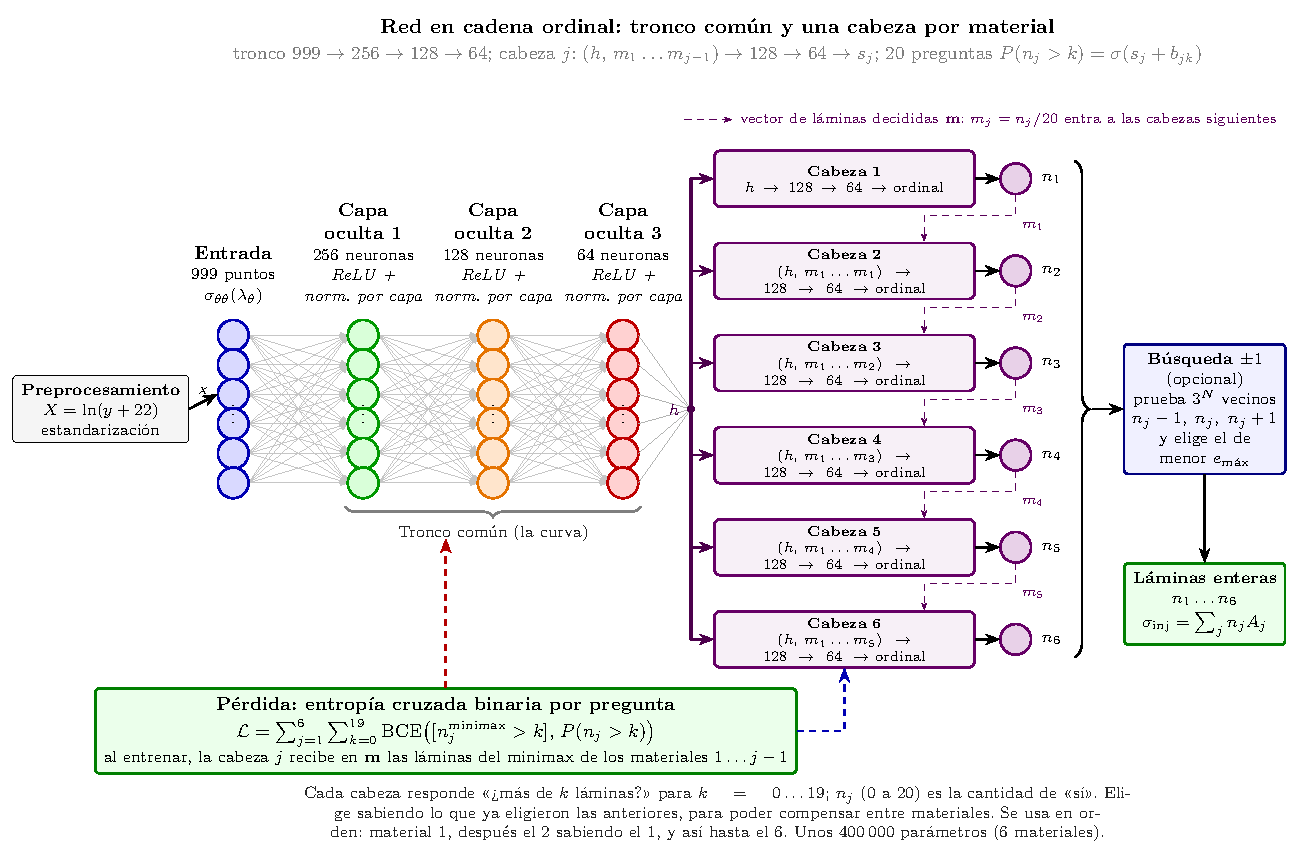
\includegraphics[width=0.95\textwidth]{red_cadena_es.pdf}
\caption{Red en cadena para $N=6$. El tronco común resume la curva en $h$; la cabeza $j$ recibe $h$ y los coeficientes ya elegidos ($m_i=z_i/20$) y responde las 20 preguntas ``¿más de $k$?''; su coeficiente es la cantidad de respuestas afirmativas. La revisión de $\pm1$, opcional, evalúa las combinaciones vecinas de la respuesta.}\label{fig:cadena}
\end{figure}

\subsection{Revisión de $\pm1$}
A la respuesta de la red se le aplica, opcionalmente, una revisión: se evalúan las $3^N$ combinaciones que difieren en a lo sumo una unidad en cada coeficiente (729 con $N=6$) y se elige la de menor $e_{\max}$. Es solo calcular $Az$ en cada combinación, sin optimizar.

\subsection{Dominio de validez}
La red se entrena con curvas de la familia y solo dentro de ese rango se garantiza su resultado. Antes de usarla se verifica que la curva nueva (1) tenga forma de J, es decir, que admita una aproximación no negativa con muchas rectas truncadas (40, con $E_{\mathrm{rms}}\le2$\,\%, por mínimos cuadrados no negativos~\cite{lawson}), y (2) quede dentro de la franja de curvas con que se entrenó. Si no cumple (2), la red no se usa y se resuelve el minimax~\eqref{eq:minimax}.

%=====================================================================
\section{Aplicación: la curva tensión--estiramiento arterial}\label{sec:aplic}
\subsection{Las variables con nombre físico}
Si la abscisa es el estiramiento circunferencial de una pared arterial, $x=\lambda_\theta$, y la ordenada la tensión circunferencial, $y=\sigma_{\theta\theta}$, la curva en J es la respuesta mecánica del tejido: blanda a bajo estiramiento, cuando trabajan la elastina y el músculo, y rígida a alto estiramiento, cuando se reclutan las fibras de colágeno~\cite{holzapfel,humphrey}. Con esos nombres, cada elemento del método toma un significado:
\begin{itemize}
\item \textbf{cada recta truncada es un material tipo fibra}: una fibra rizada que no tira hasta que el estiramiento la endereza, en su nudo $k_j$, y desde ahí responde con rigidez $S_j$;
\item \textbf{el primer nudo antes del intervalo} es un material que ya trabaja con la pared descargada, como la elastina, montado preestirado;
\item \textbf{cada coeficiente $z_j$ es un número de láminas} del material $j$, y el tope de 20 es un límite de fabricación;
\item \textbf{el ajuste~\eqref{eq:ajuste}} es la curva de un material compuesto por esas láminas, por ejemplo la pared de un injerto vascular que reproduce la respuesta de la arteria.
\end{itemize}

\subsection{Datos}
Masson et al.~\cite{masson} midieron en forma no invasiva el diámetro y la presión de la carótida común de 16 sujetos normotensos y 25 hipertensos, y ajustaron a cada uno un modelo de la pared con elastina, cuatro familias de fibras de colágeno y tono muscular. Con sus parámetros se calcula, para cada sujeto, $\sigma_{\theta\theta}(\lambda_\theta)$ en el borde media--adventicia en $n=999$ puntos de $[1{,}02;\,1{,}16]$. Las 41 curvas son J y van de 4,7 a 49\,kPa al comienzo y de 54 a 290\,kPa al final (Fig.~\ref{fig:sigma}). Diez sujetos se reservan para prueba y no intervienen en ninguna elección del método. Dos curvas límite, $y_1$ e $y_2$, encierran a los 41 y definen la familia: las curvas de trabajo y de entrenamiento se generan dentro de esa franja, que es el dominio de validez de la red.

\begin{figure}[tb]\centering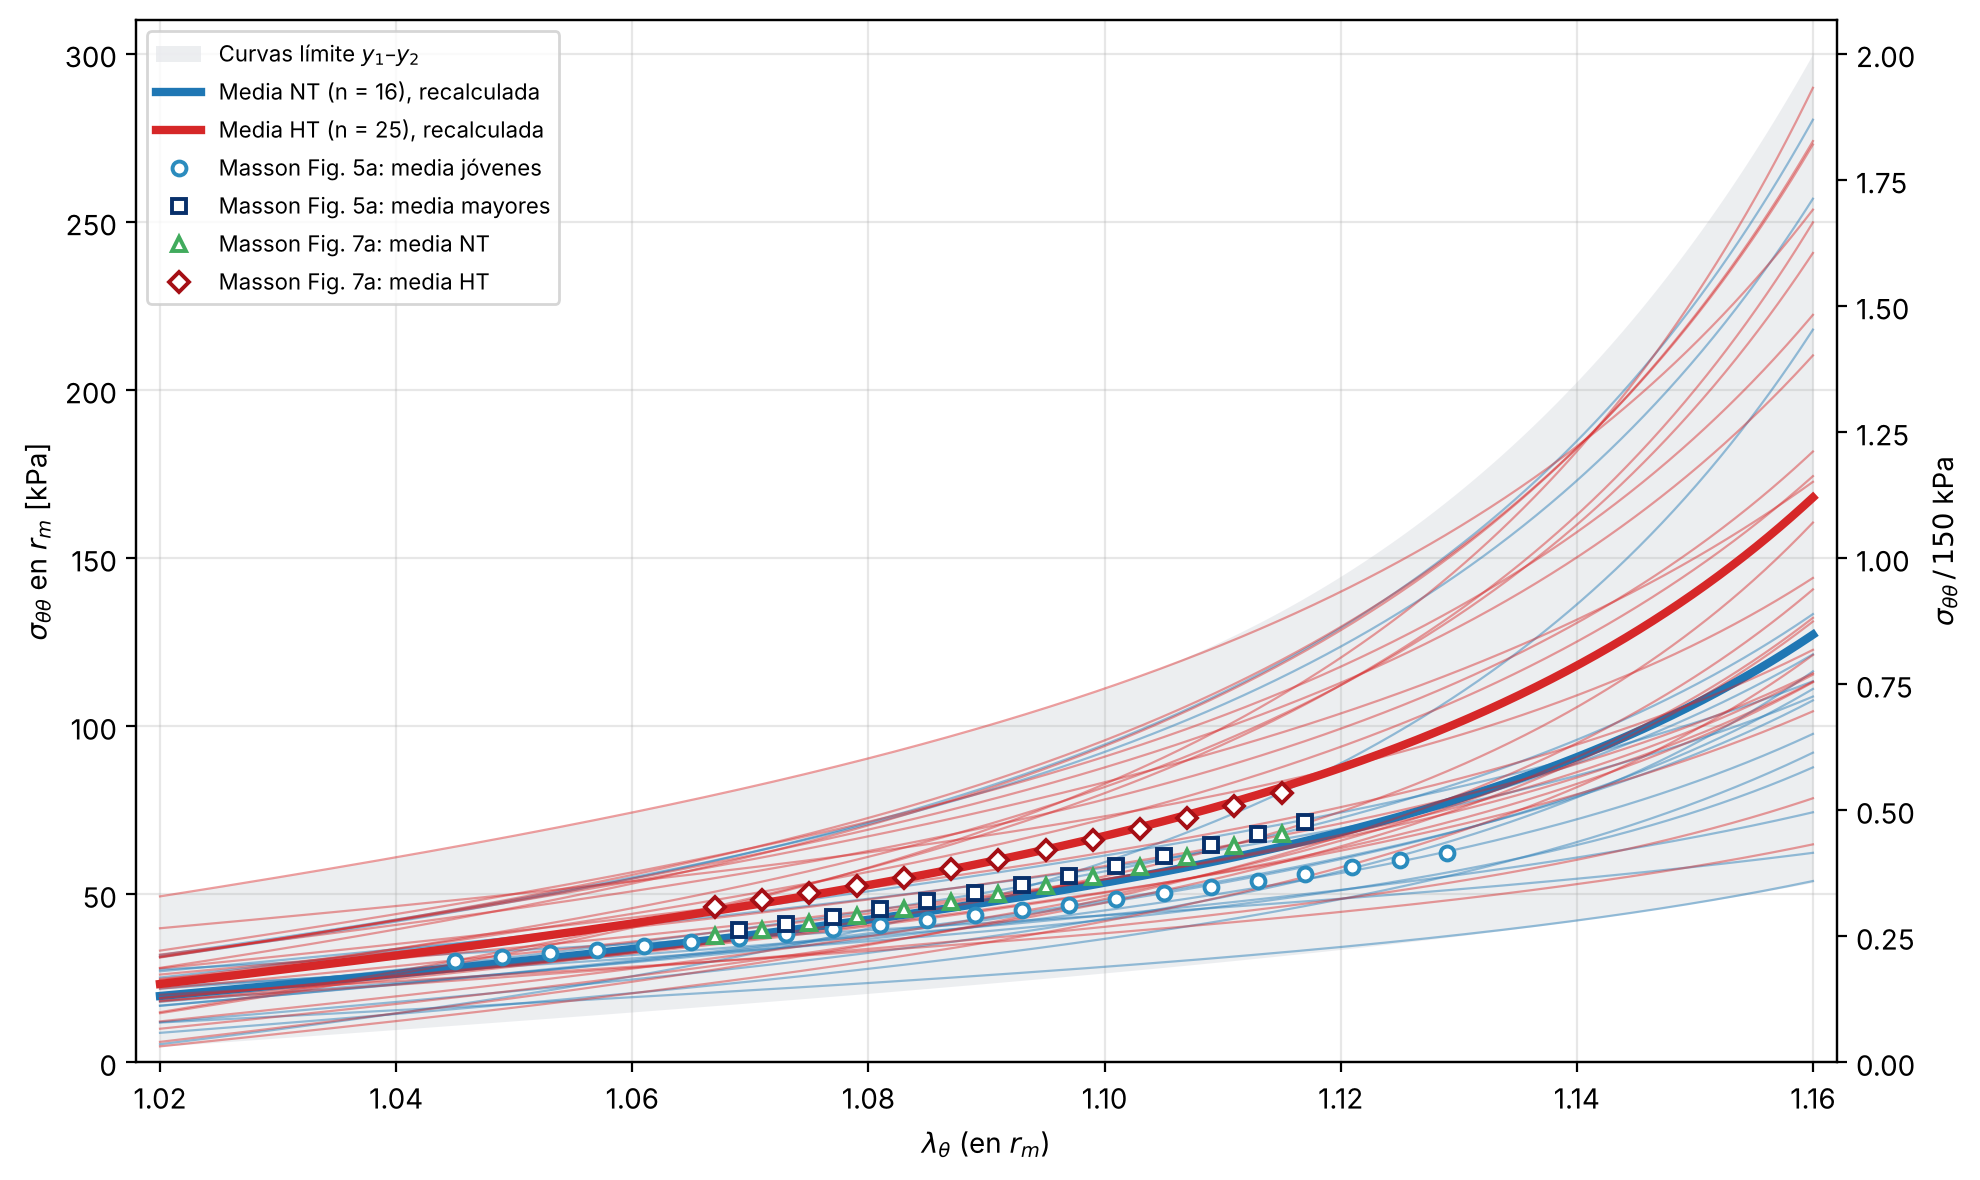
\includegraphics[width=0.74\textwidth]{fig1_sujetos_sigma_v49.png}
\caption{Las 41 curvas de Masson et al.\ (eje izquierdo en kPa; eje derecho, relativo a 150\,kPa). Franja gris: curvas límite $y_1$--$y_2$, el dominio de validez. Azul: normotensos; rojo: hipertensos.}\label{fig:sigma}\end{figure}

\subsection{La base obtenida}
La Tabla~\ref{tab:bases} y la Fig.~\ref{fig:bases} muestran las bases de 6 y de 5 rectas. Los números de condición son 28,0 y 19,0, y ninguna curva de la familia necesita un coeficiente negativo. Con coeficientes reales, el ajuste cumple la meta en todas las curvas de trabajo y en los 41 sujetos, con un peor error de 0,88\,\% (6 rectas) y 1,41\,\% (5).

\begin{table}[tb]\centering\small
\caption{Bases adoptadas: nudos $k_j$ y pendiente de una unidad $S_j$ [kPa].}\label{tab:bases}
\begin{tabular}{lcccccc}\toprule
 & 1 & 2 & 3 & 4 & 5 & 6\\\midrule
$N=6$, $k_j$ & 0,8193 & 1,0227 & 1,0774 & 1,1099 & 1,1318 & 1,1478\\
\phantom{$N=6$, }$S_j$ & 12,32 & 41,39 & 34,73 & 57,79 & 83,23 & 111,13\\\addlinespace
$N=5$, $k_j$ & 0,8228 & 1,0243 & 1,0881 & 1,1226 & 1,1447 & ---\\
\phantom{$N=5$, }$S_j$ & 12,56 & 43,57 & 51,92 & 88,74 & 129,08 & ---\\\bottomrule
\end{tabular}
\end{table}

\begin{figure}[tb]\centering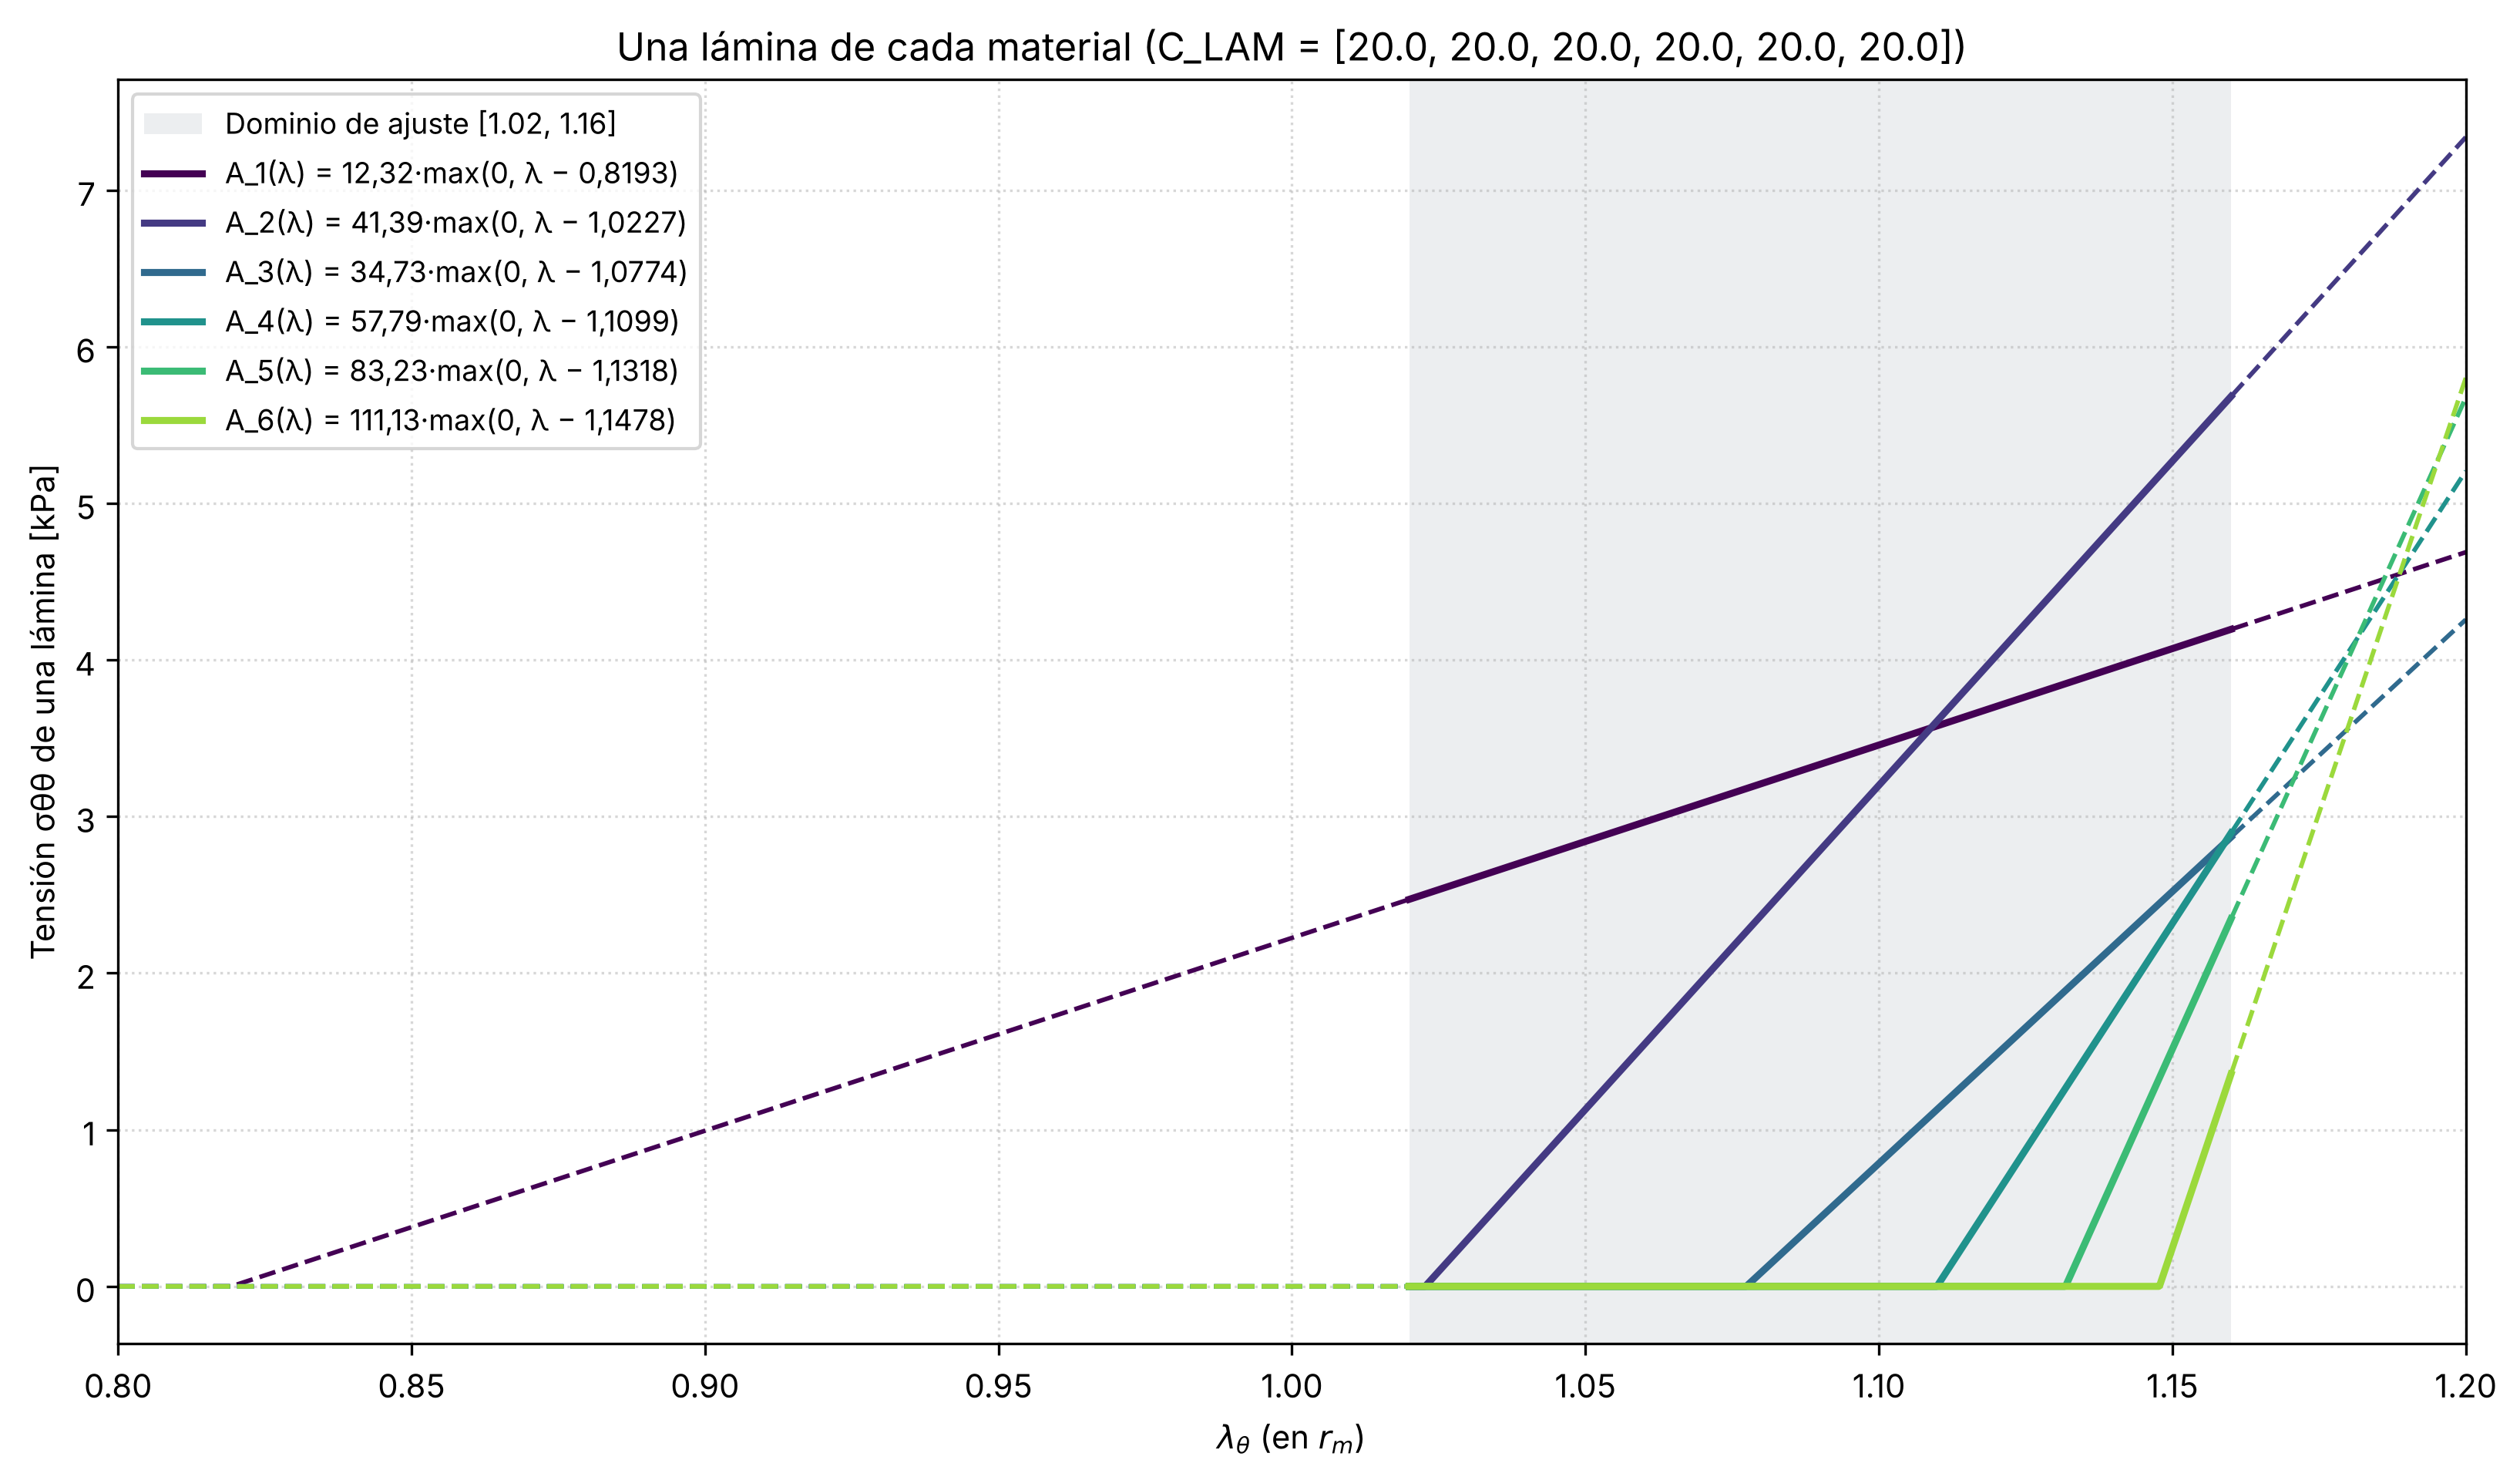
\includegraphics[width=0.6\textwidth]{bases_funcionales_v39_6.png}
\caption{La base de 6 rectas: una unidad de cada una. El primer nudo está antes del intervalo; los demás se agrupan donde la curva se curva más.}\label{fig:bases}\end{figure}

\subsection{Entrenamiento}
Se generaron 50\,000 curvas en siete familias: tres de la ley de Masson con parámetros de los sujetos de entrenamiento mezclados, perturbados o sorteados en su rango; otra ley exponencial; los 31 sujetos de entrenamiento; y dos familias de sumas de la propia base. Se conservan las 34\,503 que quedan dentro de la franja $y_1$--$y_2$, separadas en 24\,151 de entrenamiento, 3451 de validación y 6901 de prueba. A la entrada se le suma un ruido de 1\,\%, y la respuesta correcta de cada curva son sus coeficientes minimax. La entrada es $\ln(y+22)$, estandarizada punto a punto. El entrenamiento usa Adam~\cite{adam} y TensorFlow~\cite{tf}, y tarda unos 16 minutos de CPU.

%=====================================================================
\section{Resultados}
La Tabla~\ref{tab:resumen} resume los resultados con 6 rectas, por separado para las curvas que la red vio al entrenarse, las de prueba, 2000 curvas de la familia y 63 curvas de otros tres estudios.

\begin{table}[tb]\centering\small
\caption{$N=6$, coeficientes enteros: $e_{\max}$ mediano / peor [\%] · curvas que cumplen la meta (3\,\%; 4\,\% en las 2000 curvas de la familia). Errores contra la curva original.}\label{tab:resumen}
\begin{tabular}{lccc}\toprule
Conjunto & Minimax (referencia) & Red en cadena & Red + revisión $\pm1$\\\midrule
Masson, entrenamiento (31) & 1,01 / 2,34 · 31 & 1,26 / 2,34 · 31 & 1,09 / 2,34 · 31\\
Masson, prueba (10) & 1,04 / 1,61 · 10 & 1,27 / 2,82 · 10 & 1,07 / 1,61 · 10\\
Curvas de la familia (2000) & 1,06 / 3,28 · 2000 & 1,22 / 4,93 · 1998 & 1,10 / 4,93 · 1999\\
Otros estudios (63) & 1,91 / 5,71 · 57 & 2,26 / 9,44 · 46 & 2,12 / 6,16 · 50\\\bottomrule
\end{tabular}
\end{table}

\begin{itemize}
\item \textbf{Curvas de prueba.} La red ajusta dentro de la meta los 10 sujetos de prueba, sola y con la revisión de $\pm1$; en este último caso, su peor error es igual al del minimax (1,61\,\%).
\item \textbf{Otros estudios.} Sin cambiar nada ---la misma base, la misma red, la misma franja---, el método se aplicó a curvas de carótidas común, externa e interna recalculadas con las leyes y los parámetros publicados por Sommer y Holzapfel~\cite{sommer}, Liu et al.~\cite{liu} y Kamenskiy et al.~\cite{kamenskiy}. Cada curva se llevó al intervalo $[1{,}02;\,1{,}16]$ con un cambio afín de la abscisa, sin tocar la ordenada. De 98 curvas, 63 quedan dentro de la franja. La red con revisión cumple en 50 y el minimax en 57. En las 6 restantes ningún ajuste entero cumple: son curvas casi rectas y de poco recorrido, en las que una sola unidad mueve el ajuste más de lo que permite la meta.
\item \textbf{Varios ajustes enteros casi equivalentes.} La red da exactamente los coeficientes del minimax en 6 de los 41 sujetos, pero donde difiere lo hace en una o dos unidades con errores parecidos. Por eso la red se juzga por el error del ajuste y no por coincidir con el minimax.
\item \textbf{Tiempo.} El minimax tarda de 50 a 65\,ms por curva. La red, en lote, 0,3\,ms por curva, y con la revisión de $\pm1$, 2,0\,ms: de 30 a 200 veces menos.
\end{itemize}

\begin{figure}[tb]\centering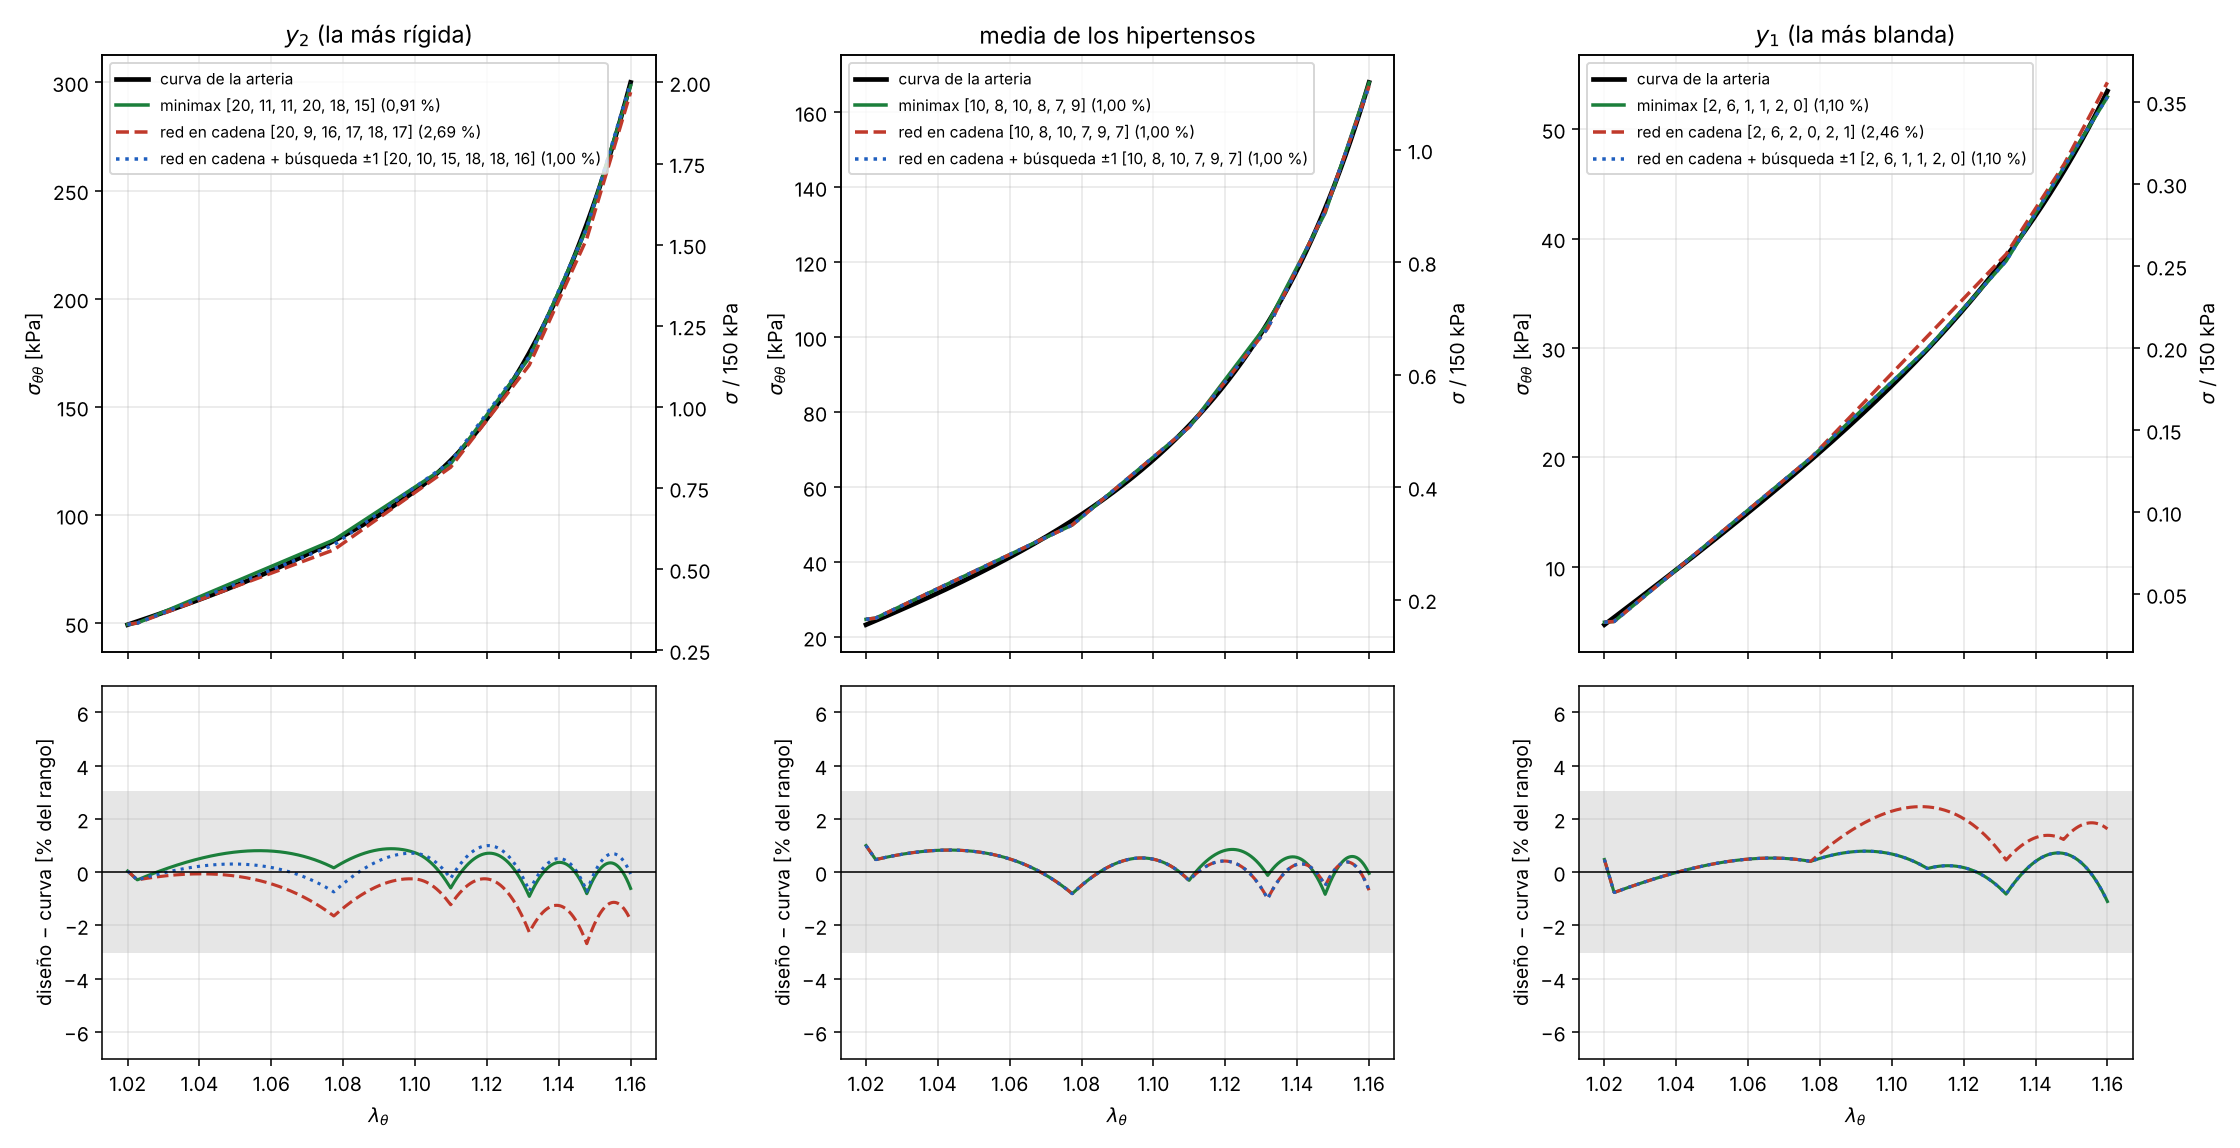
\includegraphics[width=0.9\textwidth]{v58_limite_es.png}
\caption{$N=6$: la curva más rígida de la franja ($y_2$), la media de los hipertensos y la más blanda ($y_1$). Arriba: la curva y sus ajustes, con los coeficientes de cada uno y su $e_{\max}$; abajo: ajuste $-$ curva en \% del rango (franja gris: meta de $\pm3$\,\%).}\label{fig:limite}\end{figure}

\begin{figure}[tb]\centering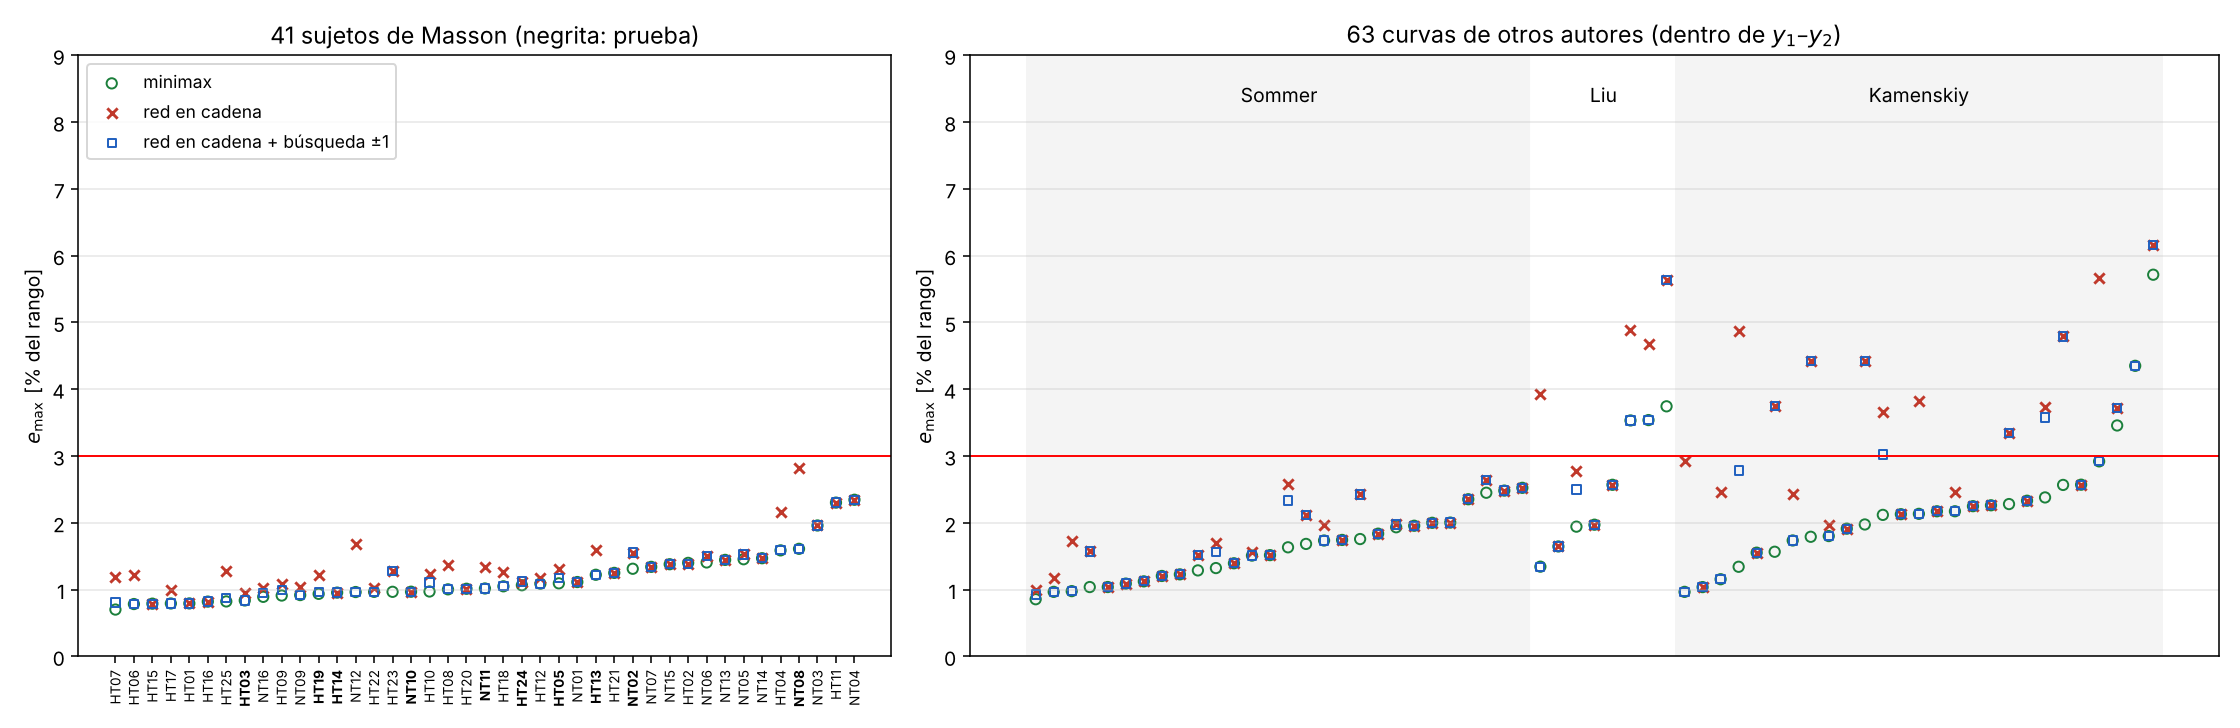
\includegraphics[width=0.9\textwidth]{v58_emax_es.png}
\caption{Peor error de cada curva con coeficientes enteros, $N=6$: minimax (círculos), red en cadena (cruces) y red con revisión de $\pm1$ (cuadrados). Izquierda: los 41 sujetos (en negrita, los de prueba). Derecha: las 63 curvas de otros estudios. Línea roja: meta de 3\,\%.}\label{fig:emax}\end{figure}

%=====================================================================
\section{Procedimiento para ajustar una curva medida}
\begin{caja}{Ajuste de una curva nueva $y(x)$}
\begin{enumerate}[label=\arabic*.]
\item \textbf{Llevar la curva al intervalo de trabajo} con un cambio afín de la abscisa (aquí, $[1{,}02;\,1{,}16]$ en 999 puntos), sin tocar la ordenada.
\item \textbf{Verificar que esté en el dominio de validez}: que tenga forma de J y que quede dentro de la franja de la familia.
\item \textbf{Evaluar la red}: $N$ evaluaciones en cadena dan los coeficientes.
\item \textbf{Revisar $\pm1$} y quedarse con la combinación de menor $e_{\max}$.
\item \textbf{Comprobar} $e_{\max}\le3$\,\% contra la curva. Si la curva no cumple el paso 2, la red no se usa y se resuelve el minimax~\eqref{eq:minimax}.
\end{enumerate}
El resultado es
\[
y(x)\approx\sum_{j=1}^{N}z_j\,S_j\,\max(0,\ x-k_j),
\]
con $k_j$ y $S_j$ fijos (Tabla~\ref{tab:bases}) y $z_j$ enteros de 0 a 20.
\end{caja}

%=====================================================================
\section{Alcances y límites}
\begin{itemize}
\item \textbf{Clase de curvas.} El método ajusta curvas crecientes y convexas. Una curva que no tiene forma de J no admite un buen ajuste con coeficientes no negativos y se rechaza en el paso 2.
\item \textbf{Dónde vale la red.} Solo dentro de la franja de la familia con que se entrenó. Otra familia de curvas requiere otra base, otra franja y otro entrenamiento; el procedimiento es el mismo.
\item \textbf{El techo de los enteros.} En curvas de muy poco recorrido, la división en 20 unidades por coeficiente no alcanza para la meta, ni con el minimax. Con coeficientes reales se ajustan todas: el límite lo pone la cuantización, no la base ni la red.
\item \textbf{Curvas con ruido.} Las curvas de prueba y de los otros estudios están recalculadas con leyes ajustadas, sin ruido de medición. El minimax minimiza el peor punto, y en una medición con ruido ese punto puede ser un pico de ruido. La red se entrenó con un ruido de 1\,\% en la entrada, pero el efecto del ruido de medición sobre el ajuste no se evaluó en este trabajo. Con una curva medida conviene suavizarla antes de ajustarla.
\end{itemize}

\section{Conclusión}
Una curva en J se ajusta con una suma de rectas truncadas de una base fija y coeficientes enteros no negativos. El ajuste es creciente y convexo por construcción. La base se elige una vez para toda una familia de curvas, con criterios de precisión en las peores curvas, condicionamiento y signo. El ajuste minimax da los mejores coeficientes enteros que existen, y con él se entrena una red neuronal que da los coeficientes de una curva nueva en una evaluación. En las curvas tensión--estiramiento de 41 carótidas, la red, con una revisión de $\pm1$, ajusta dentro de la meta los 10 sujetos de prueba y 50 de 63 curvas de otros estudios; en total, 91 de los 98 casos que admiten un ajuste entero dentro de la meta (el 93\,\%), sin resolver ninguna optimización.

\begin{thebibliography}{99}\footnotesize\setlength{\itemsep}{0pt}
\bibitem{tf} Abadi, M., et al. (2016). TensorFlow: a system for large-scale machine learning. \emph{Proc. 12th USENIX OSDI}, 265--283. \url{https://www.usenix.org/conference/osdi16/technical-sessions/presentation/abadi}
\bibitem{bengiolodi} Bengio, Y., Lodi, A., Prouvost, A. (2021). Machine learning for combinatorial optimization: a methodological tour d'horizon. \emph{Eur. J. Oper. Res.} 290, 405--421. \href{https://doi.org/10.1016/j.ejor.2020.07.063}{doi:10.1016/j.ejor.2020.07.063}
\bibitem{cao} Cao, W., Mirjalili, V., Raschka, S. (2020). Rank consistent ordinal regression for neural networks with application to age estimation. \emph{Pattern Recognit. Lett.} \href{https://doi.org/10.1016/j.patrec.2020.11.008}{doi:10.1016/j.patrec.2020.11.008}
\bibitem{cheney} Cheney, E.\,W. (1966). \emph{Introduction to Approximation Theory}. McGraw-Hill.
\bibitem{cybenko} Cybenko, G. (1989). Approximation by superpositions of a sigmoidal function. \emph{Math. Control Signals Syst.} 2, 303--314. \href{https://doi.org/10.1007/BF02551274}{doi:10.1007/BF02551274}
\bibitem{dembczynski} Dembczy\'nski, K., Cheng, W., Hüllermeier, E. (2010). Bayes optimal multilabel classification via probabilistic classifier chains. En \emph{Proc. 27th Int. Conf. Machine Learning (ICML)}. \url{https://mlanthology.org/icml/2010/dembczynski2010icml-bayes}
\bibitem{frankhall} Frank, E., Hall, M. (2001). A simple approach to ordinal classification. En \emph{Machine Learning: ECML 2001}, LNCS 2167. \href{https://doi.org/10.1007/3-540-44795-4_13}{doi:10.1007/3-540-44795-4\_13}
\bibitem{golub} Golub, G.\,H., Van Loan, C.\,F. (2013). \emph{Matrix Computations}, 4.ª ed. Johns Hopkins University Press.
\bibitem{holzapfel} Holzapfel, G.\,A., Gasser, T.\,C., Ogden, R.\,W. (2000). A new constitutive framework for arterial wall mechanics and a comparative study of material models. \emph{J. Elasticity} 61, 1--48. \href{https://doi.org/10.1023/A:1010835316564}{doi:10.1023/A:1010835316564}
\bibitem{hornik} Hornik, K. (1991). Approximation capabilities of multilayer feedforward networks. \emph{Neural Networks} 4, 251--257. \href{https://doi.org/10.1016/0893-6080(91)90009-T}{doi:10.1016/0893-6080(91)90009-T}
\bibitem{highs} Huangfu, Q., Hall, J.\,A.\,J. (2018). Parallelizing the dual revised simplex method. \emph{Math. Program. Comput.} 10, 119--142. \href{https://doi.org/10.1007/s12532-017-0130-5}{doi:10.1007/s12532-017-0130-5}
\bibitem{humphrey} Humphrey, J.\,D. (2002). \emph{Cardiovascular Solid Mechanics: Cells, Tissues, and Organs}. Springer.
\bibitem{adam} Kingma, D.\,P., Ba, J. (2015). Adam: a method for stochastic optimization. \emph{Proc. ICLR}. \url{https://arxiv.org/abs/1412.6980}
\bibitem{lawson} Lawson, C.\,L., Hanson, R.\,J. (1995). \emph{Solving Least Squares Problems}. SIAM.
\bibitem{kamenskiy} Kamenskiy, A.\,V., Dzenis, Y.\,A., MacTaggart, J.\,N., Lynch, T.\,G., Jaffar Kazmi, S.\,A., Pipinos, I.\,I. (2012). Nonlinear mechanical behavior of the human common, external, and internal carotid arteries in vivo. \emph{J. Surg. Res.} 176(1), 329--336. \href{https://doi.org/10.1016/j.jss.2011.09.058}{doi:10.1016/j.jss.2011.09.058}
\bibitem{lilin} Li, L., Lin, H.-T. (2007). Ordinal regression by extended binary classification. \emph{Advances in Neural Information Processing Systems} 19. \url{https://proceedings.neurips.cc/paper/2006/hash/019f8b946a256d9357eadc5ace2c8678-Abstract.html}
\bibitem{liu} Liu, H., et al. (2012). Using in vivo Cine and 3D multi-contrast MRI to determine human atherosclerotic carotid artery material properties and circumferential shrinkage rate and their impact on stress/strain predictions. \emph{J. Biomech. Eng.} 134, 011008. \href{https://doi.org/10.1115/1.4005685}{doi:10.1115/1.4005685}
\bibitem{masson} Masson, I., Beaussier, H., Boutouyrie, P., Laurent, S., Humphrey, J.\,D., Zidi, M. (2011). Carotid artery mechanical properties and stresses quantified using in vivo data from normotensive and hypertensive humans. \emph{Biomech. Model. Mechanobiol.} 10(6), 867--882. \href{https://doi.org/10.1007/s10237-010-0279-6}{doi:10.1007/s10237-010-0279-6}
\bibitem{nair} Nair, V., Bartunov, S., Gimeno, F., et al. (2020). Solving mixed integer programs using neural networks. arXiv:2012.13349. \url{https://arxiv.org/abs/2012.13349}
\bibitem{nelder} Nelder, J.\,A., Mead, R. (1965). A simplex method for function minimization. \emph{Computer J.} 7(4), 308--313. \href{https://doi.org/10.1093/comjnl/7.4.308}{doi:10.1093/comjnl/7.4.308}
\bibitem{nocedal} Nocedal, J., Wright, S.\,J. (2006). \emph{Numerical Optimization}, 2.ª ed. Springer, Nueva York (cap.~17: métodos de penalización).
\bibitem{penrose} Penrose, R. (1955). A generalized inverse for matrices. \emph{Math. Proc. Cambridge Philos. Soc.} 51(3), 406--413. \href{https://doi.org/10.1017/S0305004100030401}{doi:10.1017/S0305004100030401}
\bibitem{read11} Read, J., Pfahringer, B., Holmes, G., Frank, E. (2011). Classifier chains for multi-label classification. \emph{Machine Learning} 85, 333--359. \href{https://doi.org/10.1007/s10994-011-5256-5}{doi:10.1007/s10994-011-5256-5}
\bibitem{rockafellar} Rockafellar, R.\,T., Uryasev, S. (2000). Optimization of conditional value-at-risk. \emph{J. Risk} 2(3), 21--41. \href{https://doi.org/10.21314/JOR.2000.038}{doi:10.21314/JOR.2000.038}
\bibitem{sommer} Sommer, G., Holzapfel, G.\,A. (2012). 3D constitutive modeling of the biaxial mechanical response of intact and layer-dissected human carotid arteries. \emph{J. Mech. Behav. Biomed. Mater.} 5, 116--128. \url{https://www.sciencedirect.com/science/article/pii/S1751616111002177}
\bibitem{storn} Storn, R., Price, K. (1997). Differential evolution: a simple and efficient heuristic for global optimization over continuous spaces. \emph{J. Global Optim.} 11, 341--359. \href{https://doi.org/10.1023/A:1008202821328}{doi:10.1023/A:1008202821328}
\bibitem{trefethen} Trefethen, L.\,N., Bau, D. (1997). \emph{Numerical Linear Algebra}. SIAM.
\end{thebibliography}
\end{document}
